\documentclass[12pt]{article}
\usepackage{frExamplee}
\usepackage{booktabs}       % professional-quality tables
\usepackage{amsfonts}       % blackboard math symbols
\usepackage{amsmath}
\usepackage{amssymb}
\usepackage{graphicx}
\usepackage{csquotes}
\usepackage[backend=biber, style=ieee,]{biblatex}
\usepackage{setspace}
\usepackage[usenames, dvipsnames]{xcolor}
\usepackage{xspace}
\usepackage{caption}
\usepackage{subcaption}
\usepackage{listings}
\usepackage{multirow}
\usepackage{float}
\usepackage{mathrsfs}
\usepackage{wrapfig}
\usepackage{placeins}
\usepackage{algpseudocode}
\usepackage{algorithm}
\usepackage{algorithmicx}
\usepackage{hyperref}
\usepackage{calrsfs}
\usepackage{xcolor}
\lstset{
    language=Python,
    basicstyle=\scriptsize\ttfamily,
    keywordstyle=\color{blue},
    commentstyle=\color{green!50!black},
    stringstyle=\color{red},
    showstringspaces=false,
    numbers=left,
    numberstyle=\tiny,
    numbersep=5pt,
    frame=single,
    breaklines=true,
    breakatwhitespace=true,
    tabsize=4,
    captionpos=b
}
\usepackage{setspace}
\usepackage{fancyhdr} 
\fancyhf{}
\cfoot{\thepage}
\pagestyle{fancy}
\renewcommand{\headrulewidth}{0pt}%

\addbibresource{FRtemplates/frExampleRefs.bib}

\title{Measuring the Charge to Mass Ratio of the Electron}

\author{
Tony Wang\thanks{PRA Section: 3-6, October 11th} \\
\texttt{1009027447} \\
\texttt{tonyivt.wang@mail.utoronto.ca} \\
\And
Rowan Mackintosh \\
\texttt{1009306715} \\
\texttt{rowan.mackintosh@mail.utoronto.ca} \\
}
\begin{document}
\maketitle
\begin{abstract}
This experimental analysis aimed at measuring the charge-to-mass ratio of the electron by observing its motion in a magnetic field. The utilization of mathematical modeling and experimentation results ultimately led to a value in the approximated range of the universally agreed ratio, $1.89\cdot10^{11}\pm1.40\cdot10^{11}\;\left[c/kg\right]$. The possible impact of uncertainties and aberrations in electron trajectories was also investigated. Our reduction effort managed deviation from the axial magnetic field and accounted for possible external magnetic field interferences.
\end{abstract}
\section*{Introduction}
Electrons are fundamental particles that play a crucial role in diverse physical phenomena. In this experiment, we aim to determine a key property of electrons—the charge-to-mass ratio. This is accomplished by examining the motion of electrons within a magnetic field.

When a particle of mass $m$ and charge $e$ moves with velocity $v$ in a magnetic field $B$, it experiences a force $F$ that is orthogonal to both the velocity and the magnetic field \autocite{PhysRev.45.781}. This force can be quantified by the equation:

\begin{equation}
    \Vec{F} = e\Vec{v} \times \Vec{B}
    \label{eq:f}
\end{equation}

Where 
\begin{equation}
    \Vec{B}=\Vec{B}_c+\Vec{B}_e
    \label{bbb}
\end{equation}

considering both the generated field $\Vec{B}_c$ from Helmholtz coils as well as external fields $\Vec{B}_e$ such as Earth's magnetic field. Assuming that the magnetic field is constant and that the velocity is always perpendicular to the field, the particle should move in a circular orbit. During this motion, the magnetic force provides the necessary centripetal acceleration:

\begin{equation}
    evB = \frac{1}{r} m{v}^{2}
    \label{eq:evB}
\end{equation}

In our experiment, the particle reaches its velocity by acceleration through a potential difference $\Delta V$, leading to another important equation:

\begin{equation}
    e\Delta V = \frac{1}{2} m v^{2}
    \label{eq:e}
\end{equation}

Using these equations, the curvature of the electron orbit can be described in relation to the potential difference, magnetic field, and the mass and charge of the electron:

\begin{equation}
    \frac{1}{r} = \sqrt{\frac{e}{2m}} \frac{B}{\sqrt{\Delta V}}
    \label{eq:1r}
\end{equation}

where $r$ is the radius of the closed circular orbit exhibited by the electron. Since the two Helmholtz coils are positioned parallel at one radius away, we can relate $B_c$ to $I$. And with substitution into equation (\ref{eq:1r}):

\begin{equation}
    B_c=\left(\frac{4}{5}\right)^\frac{3}{2}\frac{\mu_0nI}{R}\implies \frac{1}{r} = \sqrt{\frac{e}{2m}} \frac{\left(\frac{4}{5}\right)^\frac{3}{2}\frac{\mu_0nI}{R}+B_e}{\sqrt{\Delta V}}
    \label{eq:bc}
\end{equation}

Then, we can define the proportionality constant $I_0$:

\begin{equation}
    I_0=\frac{B_e}{k} \text{ where } k=\frac{\mu_0n}{R\sqrt2}\left(\frac{4}{5}\right)^\frac{3}{2}
    \label{eq:i0}
\end{equation}

Combining equations (\ref{eq:bc}) and (\ref{eq:i0}), with rearrangement, we finally arrive at the two representations of the charge-mass ratio:

\begin{equation}
    \boxed{\frac{e}{m}=\left[\frac{\sqrt{\Delta V}}{kr\left(I+\frac{I_0}{\sqrt2}\right)}\right]^2}
    \label{eq:em}
\end{equation}

Or alternatively,

\begin{equation}
    \boxed{\frac{e}{m}=\frac{2\Delta V}{r^2(B_c+B_e)^2}}
    \label{eq:em2}
\end{equation}

However, we are still missing a piece of the puzzle: $B_e$, which we can find by substituting equation (\ref{bbb}) into (\ref{eq:1r}). We find out that $B_c$ varies linearly with $\frac{1}{r}$, where $\alpha$ is some constant. Hence, we are able to derive the value of $B_e$ as the negative of the y-intercept:

\begin{equation}
    B_c=\alpha\frac{1}{r}-B_e
\end{equation}

\section*{Method}
\begin{figure}[t!]
\centering
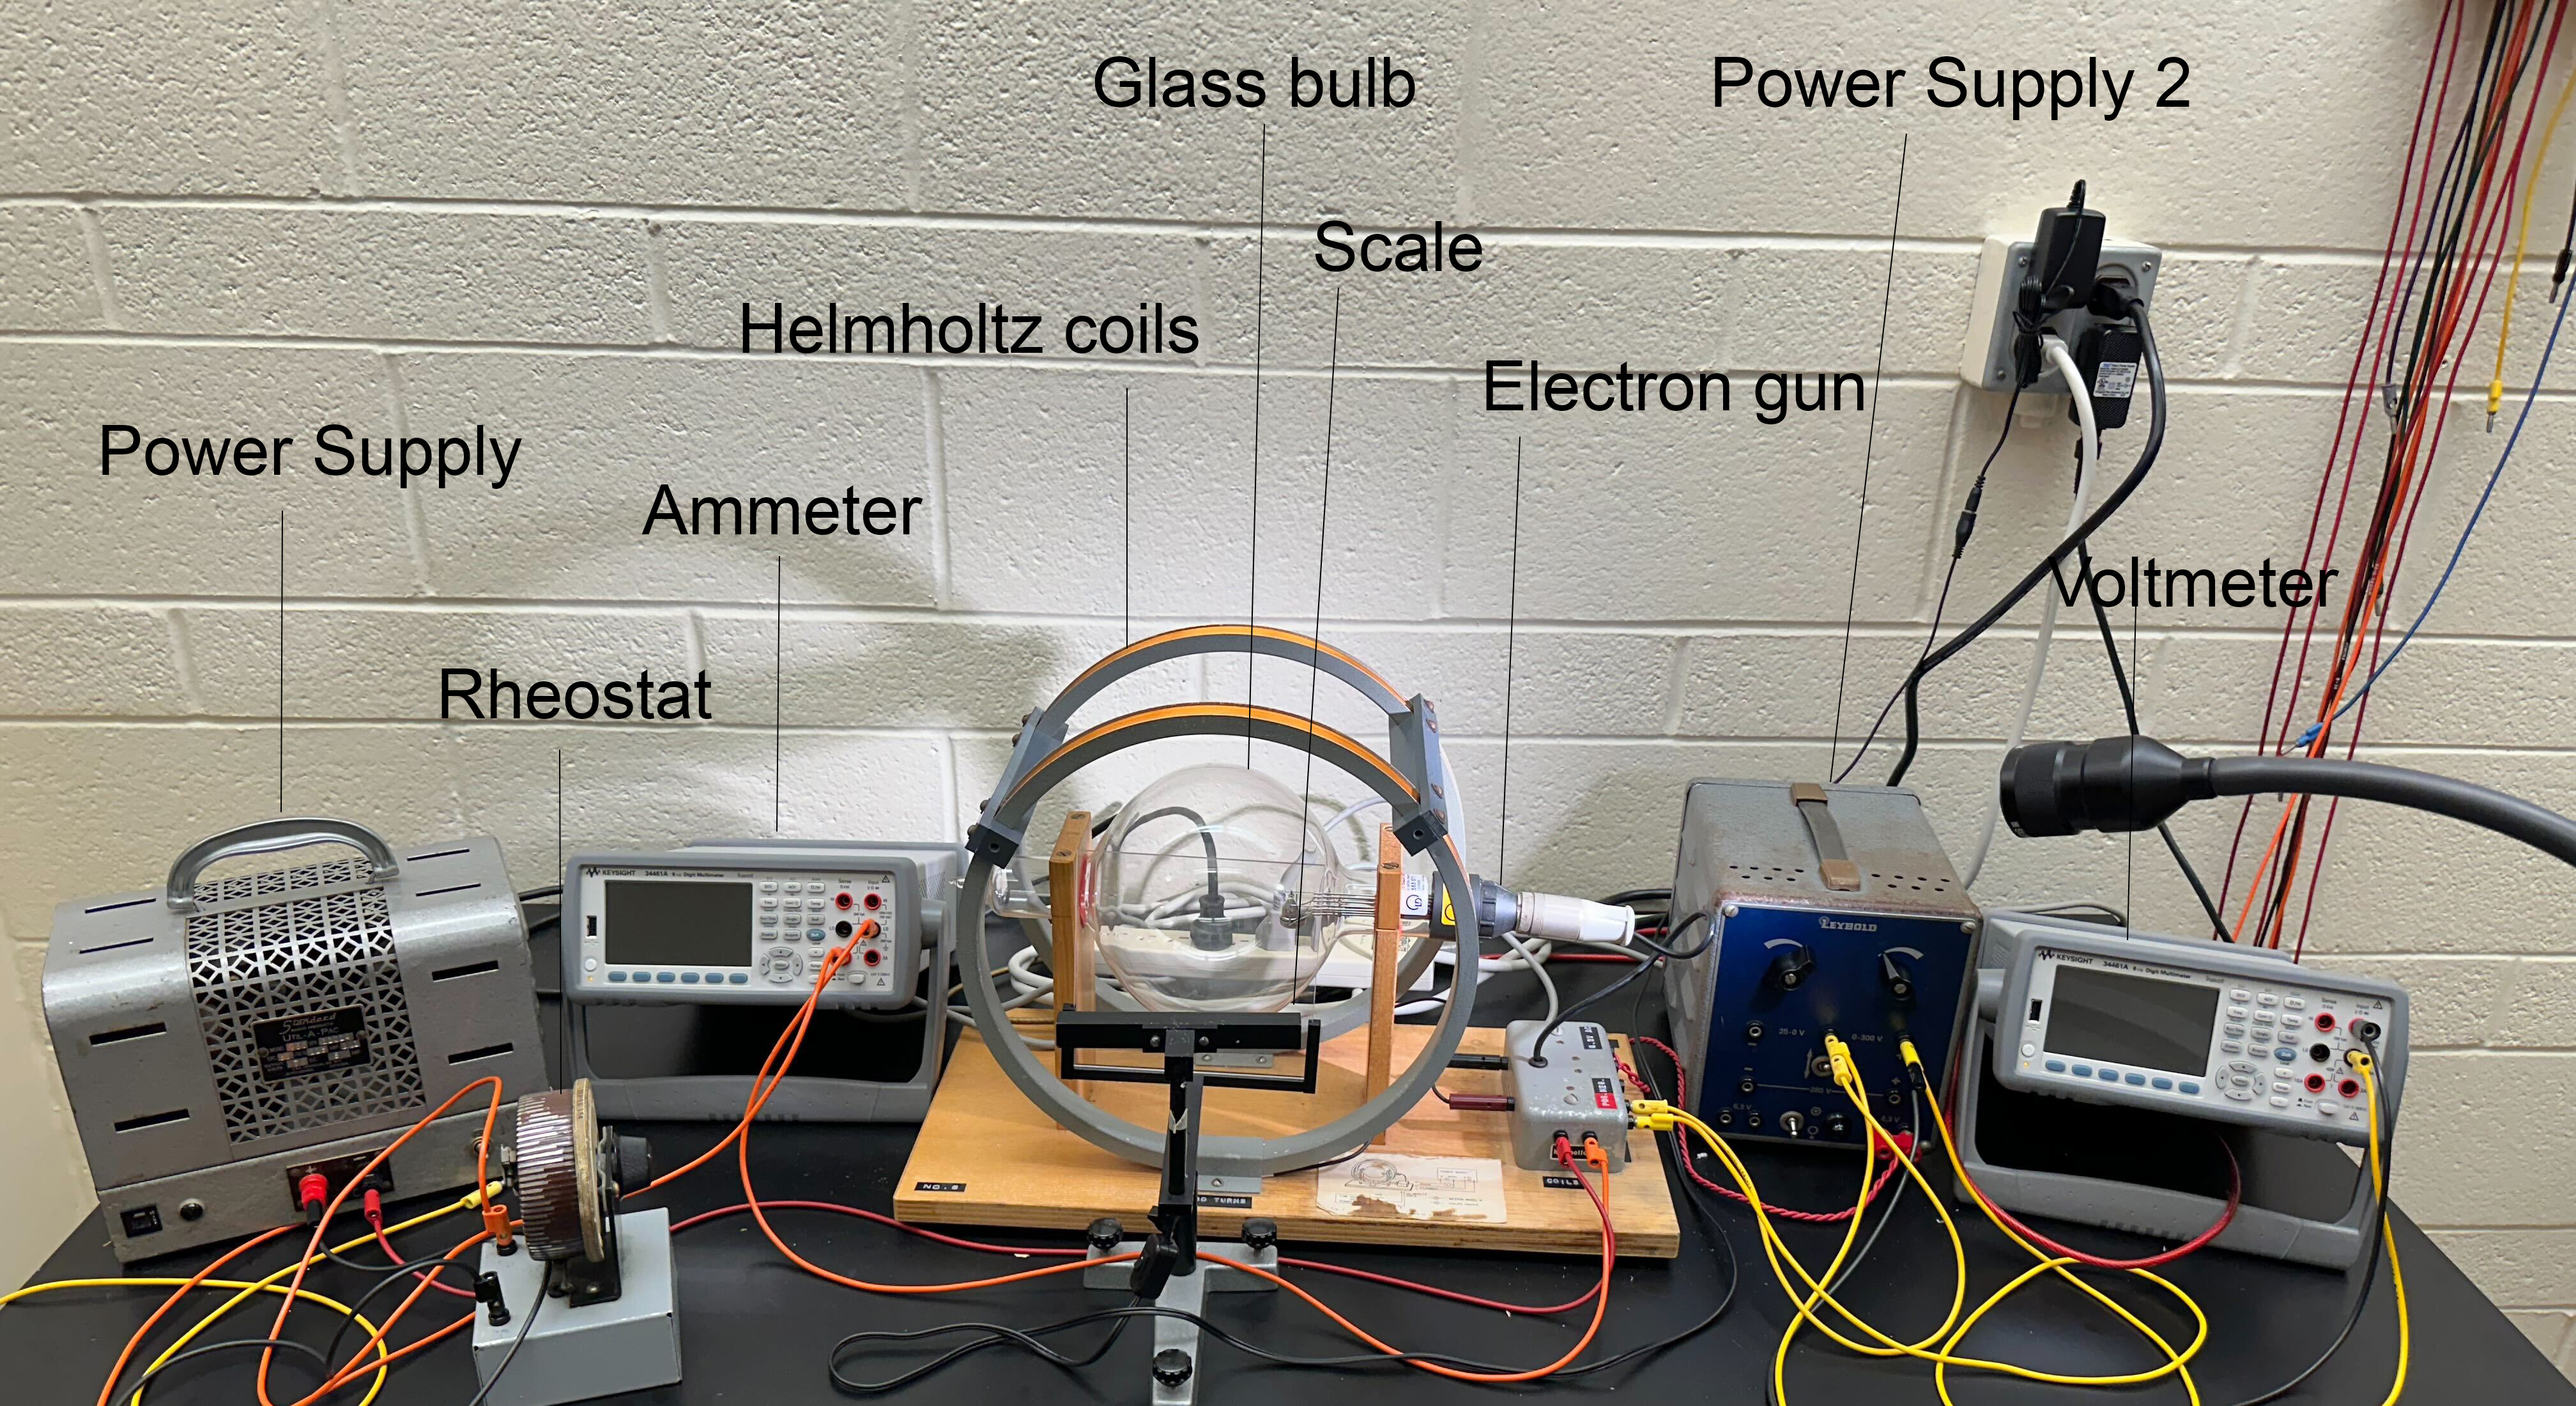
\includegraphics[width=0.65\columnwidth]{figure/aparatus.jpg}
\caption{Labelled experimental setup}
\label{fig:aparatus}
\end{figure}
\subsection*{Equipment and Associated Uncertainties}
Relevant equipment is labeled in Fig. ???\ref{fig:aparatus}
\begin{enumerate}
    \item Ammeter (uncertainty ±0.1\pm 0.1) \autocite{manualkey}
    \item Electron gun
    \item Glass bulb filled with H2{\rm H_2}
    \item Helmholtz coils, n=130,R=0.16±0.005±0.005[m]n=130,\;R=0.16 \pm 0.005 \pm 0.005\;[m]
    \item Power management box with 8 banana cables
    \item Current power source (8V DC)
    \item Rheostat
    \item Scale (uncertainty ±0.1\pm 0.1)
    \item Voltage power source (300V DC)
    \item Voltmeter (uncertainty ±0.05\pm 0.05) \autocite{manualkey}
\end{enumerate}

\subsection*{Experimental Procedure}
\begin{enumerate}
    \item Connect the apparatus as shown in Fig. ???\ref{fig:aparatus}.
    \item Power up the electron gun filament, leaving it on for 30 seconds, and then turn on the anode voltage.
    \item Activate the Helmholtz coils power supply.
    \item Ensure the electron beam is visible, maintaining a smooth trajectory.
    \begin{enumerate}
        \item Adjust the bulb rotation to prevent beam contact with the glass.
        \item Ensure the electron trajectory forms a vertical circle.
    \end{enumerate}
    \item Measure path diameters using the self-illuminated scale and plastic reflector. Familiarize yourself with the scale beforehand to avoid parallax errors.
    \item Collect data for two scenarios: constant accelerating potential and constant coil current. Record values with units and uncertainties.
\end{enumerate}

\section*{Results and Discussion}
\begin{figure}[t!]
\centering
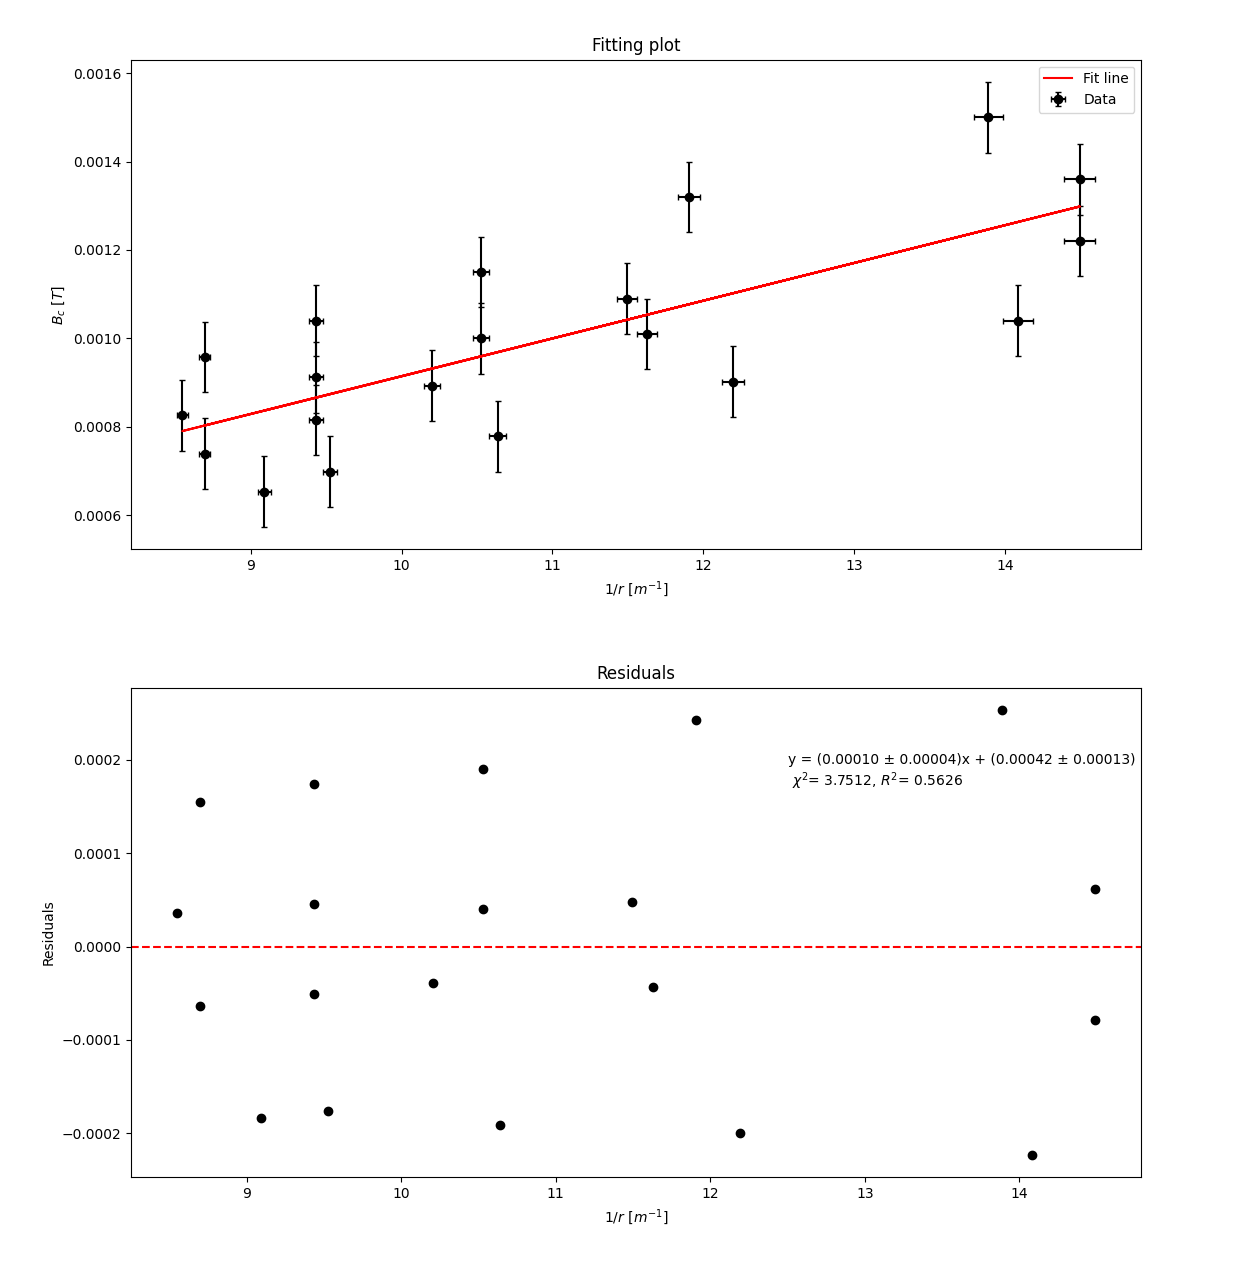
\includegraphics[width=0.8\columnwidth]{figure/Figure_1.png}
\caption{Plotted relationships between generated magnetic field, BcB_c and 1r\frac{1}{r}. Equation of fit for the line and χ2,R2\chi^2,\;R^2 are calculated and shown on the graph.}
\label{fig:subplot}
\end{figure}
All recorded experimental measurements and associated calculated values are recorded in Table \ref{table}. The plot is shown in Fig. \ref{fig:subplot}, where $\chi^2=3.7512,\;R^2=0.5626$. The values are not perfect but still indicate a valid relationship. This blame is taken by the uncertainties and sources of errors present, namely problems of parallax. We made sure that the scale and reflector stayed stationary throughout the lab for consistency, and ensured that the stand is neither leaned nor tilted such that it is always parallel. This should minimize most problems related to taking measurements, however, it is not humanly possible to ensure a perfect observation of results. Other possible errors include the lack of a vacuum in the globe, where gas particles may alter the motion of electrons.

Calculated by the python program included in the appendix, the equation of best fit is $y=0.00010\pm0.00014+0.00042\pm0.00013$. Hence, we can interpolate $B_e$ as the negative of the intercept, $-0.00042\pm0.0013\;[T]$. This negative value may not make much sense, and its value is quite a bit off from Earth's average magnetic field of around $0.000025$ to $0.000065\;[T]$, but when we consider the uncertainties calculated, the actual values do fall within range \autocite{rockenbauer2001two-dimensional}. With this final piece, we can then compute the charge to mass ratio using equation (\ref{eq:em}), yielding a calculated value of $1.89\cdot10^{11}\pm1.40\cdot10^{11}\;\left[c/kg\right]$. This is close to the universally agreed ratio of $1.76\;\left[c/kg\right]$ and it falls within the range of the uncertainties \autocite{PhysRev.45.781}. Alternatively, we can also compute the ratio using equation (\ref{eq:em2}), yielding a very similar value of $1.88\cdot10^{11}\pm1.40\cdot10^{11}\;\left[c/kg\right]$.

On the topic of uncertainties, we investigate the behavior of the electron trajectory, particularly under conditions of low accelerating voltage and high magnetic field strength. Under these challenging conditions, the electron's trajectory deviates, exhibiting anomalous behavior— a divergence from the expected perfect circular path established by theoretical models \autocite{rockenbauer2001two-dimensional}. This aberration complicates the precise observation of the electron ring's radius, which is reflected in the smallest recorded values for $R$ in Table 1, tapering off around 0.07 m. Unequal distribution of magnetic force across the trajectory leads to inconsistent deflection \autocite{manson2022impact}. Such randomness introduces a degree of uncertainty in the recorded measurements, visible as discrepancies in the recorded radius measurements. Considering multiple measurements can alleviate the variable deflection issues, hewing closer to an accurate representation of the trajectory. The values obtained for $e/m$ and $B_e$ could also require a correction aimed at the magnetic field's decreased strength away from the axis known as off-axis distance correction \autocite{janes1966anomalous},
\begin{equation}
    \frac{B(\rho)}{B(0)}=1-\frac{\rho^4}{R^4\left(0.6583+0.29\frac{\rho^2}{R^2}\right)^2}
\end{equation}
where $\rho$ is the distance from the axis, which is equal to $r$ in our case. This correction factor is calculated and shown in Table \ref{table}, and applying it reduces errors to a reasonable extent. At differing levels of intensity, relativistic effects at high electron velocities, uneven gas distribution, and alignment of the experimental setup could play significant roles in the observed anomalous behavior. Therefore, careful interpretation of data, coupled with a comprehensive correction mechanism, gives valuable insights into the behavior in question and refines the results.

Another error we may be interested in considering is magnetic fields generated by nearby electronic devices, wall circuits and ferromagnetic materials etc.. While we noticed no difference coiling up the banana plug wires with a few amps running through them near the bulb, and a cellphone for sure yielded no visible difference, the impacts may still be present, just at levels below our uncertainties in the first place. Or the power lines and wall circuits in the room were already interfering with the experiment, and we would just be unable to identify any differences.

\section*{Conclusion}
To conclude, this experiment succeeded in estimating the charge-to-mass ratio of an electron, providing a value in close agreement with the universally accepted ratio.  In the end we arrived at a charge-mass ratio of $1.89\cdot10^{11}\pm1.40\cdot10^{11}\;\left[c/kg\right]$, well within range with the theoretical value when considering uncertainties. We identified sources of error, with primary ones attributed to parallax, intentional and unintentional magnetic field interference, and inhomogeneous distribution of the components, among others. The challenges and divergences in measurements also verify the complexities in precise objective measurement due to human constraints. The outcomes of this experiment should lay the groundwork for improved experimental designs and procedures for future investigations.
\newpage
\printbibliography
\section*{Appendix}
{\bf Uncertainty Propagation Formulae}
\begin{align*}
    &B_{cu}=B_c\sqrt{\left(\frac{I_u}{I}\right)^2+\left(\frac{R_u}{R}\right)^2}\\
    &\frac{B(\rho)}{B(0)}_u=8\frac{B(\rho)}{B(0)}\sqrt{\left(\frac{\rho_u}{\rho}\right)^2+\left(\frac{R_u}{R}\right)^2}\\
    &\frac{e}{m}_u=\frac{e}{m}\sqrt{\left(\frac{V_u}{V}\right)^2+\left(\frac{2r_u}{r}\right)^2+\left(\frac{2\sqrt{B_{cu}^2+B_{eu}^2}}{B_c+B_e}\right)^2}
\end{align*}
Note that the uncertainties for $B_e$ are computed with scipy in the python script provided.\\
{\bf Table for recorded data and calculated values}
\begin{table}
    \centering
    \vspace{10pt}
        \begin{tabular}{|c|c|c|c|c|}
            \hline
            V $[V]$  ± 0.05 & I $[A]$ ± 0.1 & $r$  ± 0.0005 & $B_c [T]$ & $\frac{B_c(\rho)}{B_c(0)}$\\
            \hline
            144.5 & 1.4 & 0.071 & 0.00104 ± 0.00008 & 0.9 ± 0.1  \\
            144.5 & 1.2 & 0.082 & 0.000902 ± 0.00008 & 0.9 ± 0.1   \\
            144.5 & 1.1 & 0.094 & 0.000778 ± 0.00008 & 0.8 ± 0.1   \\
            144.5 & 1.0 & 0.105 & 0.000698 ± 0.00008 & 0.70 ± 0.09   \\
            144.5 & 0.9 & 0.110 & 0.000653 ± 0.00008 & 0.65 ± 0.08   \\
            \hline
            190.6 & 1.7 & 0.069 & 0.00122 ± 0.00008 & 0.9 ± 0.1  \\
            190.6 & 1.4 & 0.086 & 0.00101 ± 0.00008 & 0.8 ± 0.1  \\
            190.6 & 1.2 & 0.098 & 0.000893 ± 0.00008 & 0.8 ± 0.1   \\
            190.6 & 1.1 & 0.106 & 0.000815 ± 0.00008 & 0.69 ± 0.09   \\
            190.6 & 1.0 & 0.115 & 0.000739 ± 0.00008 & 0.59 ± 0.07   \\
            \hline
            240.0 & 1.9 & 0.069 & 0.00136 ± 0.00008 & 0.9 ± 0.1  \\
            240.0 & 1.5 & 0.087 & 0.00109 ± 0.00008 & 0.8 ± 0.1   \\
            240.0 & 1.4 & 0.095 & 0.00100 ± 0.00008 & 0.8 ± 0.1   \\
            240.0 & 1.2 & 0.106 & 0.000912 ± 0.00008 & 0.69 ± 0.09   \\
            240.0 & 1.1 & 0.117 & 0.000826 ± 0.00008 & 0.57 ± 0.07   \\
            \hline
            315.8 & 2.1 & 0.072 & 0.00150 ± 0.00009 & 0.9 ± 0.1  \\
            315.8 & 1.8 & 0.084 & 0.00132 ± 0.00008 & 0.9 ± 0.1   \\
            315.8 & 1.6 & 0.095 & 0.00115 ± 0.00008 & 0.8 ± 0.1   \\
            315.8 & 1.4 & 0.106 & 0.00104 ± 0.00008 & 0.69 ± 0.09   \\
            315.8 & 1.3 & 0.115 & 0.000958 ± 0.00008 & 0.59 ± 0.07   \\
            \hline
        \end{tabular}
    \caption{Recorded radii measurements by altering potential difference and current}
    \label{table}
\end{table}


\newpage

% \begin{lstlisting}
% import matplotlib.pyplot as plt
% import numpy as np
% from scipy.optimize import curve_fit
% from sklearn.metrics import r2_score

% potential_difference = [144.5, 144.5, 144.5, 144.5, 144.5,
%                         190.6, 190.6, 190.6, 190.6, 190.6,
%                         240.0, 240.0, 240.0, 240.0, 240.0,
%                         315.8, 315.8, 315.8, 315.8, 315.8]
% current = [1.424, 1.235, 1.065, 0.9551, 0.8934,
%            1.673, 1.381, 1.222, 1.115, 1.011,
%            1.856, 1.497, 1.372, 1.248, 1.130,
%            2.055, 1.805, 1.417, 1.311, 1.570]
% resistance = [7.1, 8.2, 9.4, 10.5, 11,
%               6.9, 8.6, 9.8, 10.6, 11.5,
%               6.9, 8.7, 9.5, 10.6, 11.7,
%               7.2, 8.4, 10.6, 11.5, 9.5]

% def rational(x, a, b):
%     x = np.abs(x)
%     # Adding a small constant, epsilon, to prevent division by zero
%     epsilon = 1e-5
%     return a / (x - b + epsilon)

% voltages = [144.5, 190.6, 240.0, 315.8]
% x_fit = np.linspace(min(current), max(current), 500)
% fig, axs = plt.subplots(4, 2, figsize=(10, 20))

% for i, voltage in enumerate(voltages):
%     indices = [j for j, val in enumerate(potential_difference) if val == voltage]
%     x = [current[j] for j in indices]
%     y = [resistance[j] for j in indices]
%     # provide initial guesses for a and b
%     popt, pcov = curve_fit(rational, x, y, p0=[max(y), min(x)])
%     residuals = y - rational(np.array(x), *popt)
%     chi = np.sum((residuals ** 2)) / len(y)
%     r2 = r2_score(y, rational(np.array(x), *popt))
%     print("For voltage: ", voltage)
%     print("Equation: y = " + str(popt[0]) + " / ( x - " + str(popt[1]) + " )")
%     print("Residuals: ", residuals.tolist())
%     print("Chi-squared: ", chi)
%     print("R-squared: ", r2)
%     x_fit = np.linspace(min(x), max(x), 500)
%     y_fit = rational(x_fit, *popt)
%     # plot original data and the fit curve
%     axs[i, 0].plot(x, y, 'o', color='r')
%     axs[i, 0].plot(x_fit, y_fit, 'g--')
%     axs[i, 0].errorbar(x, y, yerr=0.1, fmt='o', ecolor='g')
%     axs[i, 0].set_title('Voltage: ' + str(voltage))
%     axs[i, 0].set_xlabel('Current (A)')
%     axs[i, 0].set_ylabel('Radius (unitless)')
%     # Add text annotation
%     axs[i, 0].text(0.9, 0.9, f'Chi-squared: {chi:.3f}', transform=axs[i, 0].transAxes, fontsize=10, ha='right')
%     axs[i, 0].text(0.9, 0.8, f'R-squared: {r2:.3f}', transform=axs[i, 0].transAxes, fontsize=10, ha='right')
%     # plot the residuals
%     axs[i, 1].plot(x, residuals, 'o', color='b')
%     axs[i, 1].axhline(0, color='k', linewidth=0.5)
%     axs[i, 1].set_title('Residuals - Voltage: ' + str(voltage))
%     axs[i, 1].set_xlabel('Current (A)')
%     axs[i, 1].set_ylabel('Residual')
%     equation = f'y = {popt[0]:.3f} / (x - {popt[1]:.3f})'
%     # Add text annotation
%     axs[i, 1].text(0.9, 0.9, f'Chi-squared: {chi:.3f}', transform=axs[i, 1].transAxes, fontsize=10, ha='right')
%     axs[i, 1].text(0.9, 0.8, f'R-squared: {r2:.3f}', transform=axs[i, 1].transAxes, fontsize=10, ha='right')
%     axs[i, 0].text(0.65, 0.65, equation, transform=axs[i, 0].transAxes, fontsize=10, ha='right')
    
% if __name__ == '__main__':
%     plt.tight_layout()
%     plt.show()
% \end{lstlisting}
{\bf Python Script for Plotting and Error Analysis}
\begin{lstlisting}
import numpy as np
import matplotlib.pyplot as plt
from scipy.optimize import curve_fit
from scipy.stats import linregress

def linear(x, m, b):
    return m*x + b

r_values = np.array([0.071, 0.082, 0.094, 0.105, 0.110, 0.069, 0.086, 0.098, 0.106, 0.115, 0.069, 0.087, 0.095, 0.106, 0.117, 0.072, 0.084, 0.095, 0.106, 0.115])
Bc_values = np.array([0.00104, 0.000902, 0.000778, 0.000698, 0.000653, 0.00122, 0.00101, 0.000893, 0.000815, 0.000739, 0.00136, 0.00109, 0.00100, 0.000912, 0.000826, 0.00150, 0.00132, 0.00115, 0.00104, 0.000958])
errors_Bc = 0.00008 * np.ones(Bc_values.shape)
errors_r_values = 0.0005/(r_values**2)
fitting_params, pcov = curve_fit(linear, 1/r_values, Bc_values, sigma=errors_Bc, absolute_sigma=True)
errors_fitting_params = np.sqrt(np.diag(pcov))
r_values_fit = linear(1/r_values, *fitting_params)
residuals = Bc_values - r_values_fit

# chi-squared 
dof = len(r_values) - len(fitting_params) # Degree of freedom
chi_square = sum((residuals / errors_Bc)**2)
chi_square_reduced = chi_square/dof

# r-squared 
slope, intercept, r_value, p_value, std_err = linregress(1/r_values, Bc_values)


plt.figure(figsize=(10,8))

# Main plot
plt.subplot(211)
plt.errorbar(1/r_values, Bc_values, xerr=errors_r_values, yerr=errors_Bc, linestyle='None', marker='o', capsize=2, color='k', label='Data')
plt.plot(1/r_values, r_values_fit, color='r', label='Fit line')
plt.title('Fitting plot')
plt.xlabel('1/r')
plt.ylabel('Bc')

plt.legend(loc='best')

# Residual plot
plt.subplot(212)
plt.plot(1/r_values, residuals, linestyle='None', marker='o', color='k')
plt.axhline(0, color='r', linestyle='--')
plt.title('Residuals')
plt.xlabel('1/r')
plt.ylabel('Residuals')
plt.text(0.65, 0.8, 
         'y = ({0:.5f} ± {1:.5f})x + ({2:.5f} ± {3:.5f})\n $\chi^2$= {4:.4f}, $R^2$= {5:.4f}'.format(
             fitting_params[0], errors_fitting_params[0], fitting_params[1], errors_fitting_params[1], 
             chi_square_reduced, r_value**2), transform=plt.gca().transAxes)

plt.tight_layout()
plt.show()
\end{lstlisting}
\end{document}